\begin{figure}[h]
    \centering
    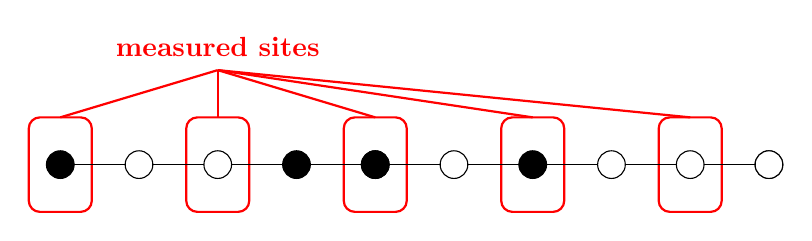
\begin{tikzpicture}[scale=1]

% Parametri
\def\nodespacing{1.0} % distanza tra i nodi
\def\numnodes{10}

% Disegna i 10 nodi
\foreach \i in {0,...,9} {
    \pgfmathparse{mod(\i,3) ? "white" : "black"}
    \edef\fillcolor{\pgfmathresult}
    \filldraw[draw=black, fill=\fillcolor] (\i*\nodespacing, 0) circle (5pt);
}

\filldraw[draw=black, fill=black] (4*\nodespacing, 0) circle (5pt);
\filldraw[draw=black, fill=white] (9*\nodespacing, 0) circle (5pt);


% Rettangoli attorno a nodi 0, 2, 4 con linea verso la scritta
\foreach \i in {0,2,4,6,8} {
    % Disegna rettangolo
    \draw[thick, red, rounded corners] 
        ({\i*\nodespacing - 0.4}, -0.6) rectangle ({\i*\nodespacing + 0.4}, 0.6);
    
    % Disegna linea che parte dal centro superiore del rettangolo
\draw[thick, red] ({\i*\nodespacing}, 0.6) -- (2*\nodespacing, 1.2);
}

% Scritta "measured" centrata sopra
\node[text=red, font=\bfseries] at (2*\nodespacing, 1.5) {measured sites};

\foreach \i in {0,...,8} {
    \draw (\i*\nodespacing + 0.17,0) -- (\i*\nodespacing + \nodespacing - 0.17,0);
    }
\end{tikzpicture}
    \caption{One-dimensional fermionic chain with local measurements applied on a finite fraction of sites.}
   % \label{fig:enter-label}
\end{figure}